\documentclass[12pt]{article}

% Language setting
\usepackage[utf8]{inputenc}
\usepackage[bulgarian]{babel}

% --------------------- Packages  --------------------
% Use biblatex
\usepackage{biblatex}
\addbibresource{bibliography.bib}
% Table thickness
\usepackage{ctable}
% Equations: SI units
\usepackage{siunitx}
% Approximately equal
\usepackage{amssymb}
% degrees symbol
\usepackage{gensymb}
% warning box
\usepackage{pifont,mdframed}
% Multiline math
\usepackage{amsmath}

\newenvironment{warning}
  {\par\begin{mdframed}[linewidth=2pt, linecolor=white]%
    \begin{list}{}{\leftmargin=1cm
                   \labelwidth=\leftmargin}\item[\Large\ding{43}]}
  {\end{list}\end{mdframed}\par}

% --------------------- Title  --------------------
\addbibresource{bibliography.bib}

\begin{document}

% Anfang der Titelseite________________________________________________________________________________
\begin{titlepage}
	\flushleft
	{\scshape\Large Протокол XI \hspace{2cm} Молекулна физика\par}
	\vspace{4cm}
	{\huge\bfseries Изчисляване на топлинен капацитет на калориметър\par}
	\vspace{1cm}
	{\LARGE\bfseries Лабораторно упражнение №3.11, задача 1\par}
	\vspace{5cm}
    {\LARGE\bfseries Виолета Кабаджова, \par}
    {\large\bfseries ККТФ, фак. номер: 3PH0600026\par}
	\vspace{1cm}
	
	{\large Физически Факултет, 
	
	Софийски Университет "Св. Климент Охридски"
	
	29 май 2023 г.\par}
	
\end{titlepage}

\section{Теоритична част}\label{sec:theoretical-part}
При изследването на топлинните капацитети на определени материали често използваме калориметър. Ако обаче неговата температурата и тази на телата, поставени в него са с различна температура, то между тях започва топлообмен (уравнение на топлинния баланс - \ref{eq:thermal-equilibrium}, където $Q_1i$ са топлините на по-топлите тела, а $Q_2i$ - на по-студените тела), който ако не бъде отчетен предизвиква значителни грешки в измерванията.

\begin{equation}\label{eq:thermal-equilibrium}
    \Sigma_i Q_{1i} = \Sigma_i Q_{2i}
\end{equation}

\begin{figure}
    \centering
    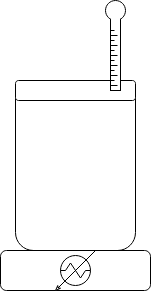
\includegraphics[width=0.2\textwidth]{images/setup-caloriemeter.drawio.png}
    \caption{\label{fig:setup}Схема на опитна постановка: калориметър върху нагревател и термометър}
    \label{fig:setup}
\end{figure}

На фиг. \ref{fig:setup} е представена принципна схема на опитната установка. Нагревателят отдава топлина, равна на $Q_1 = UIt$, където $I$ - големината на електричния ток, протичащ през нагревателя, $U$ - пада на напрежението, $t$ - времето за нагряване. Топлините, които ще погълнат съответно калориметърът и водата, са съответно $Q_{21} = C_{K}\Delta T$ и $Q_{22} = c_BM_B \Delta T$, където $\Delta T = (T_1 - T_0)$ ($T_1$ - температура в края на загряването, $T_0$ - температура в началото на загряването), $c_B$ - специфичен топлинен капацитет на водата, $M_B$ - маса на водата. От ур. \ref{eq:thermal-equilibrium} следва уравнение \ref{eq:thermal-equation-work-formula}, откъдето и работната ни формула \ref{eq:work-formula}.

\begin{equation}\label{eq:thermal-equation-work-formula}
    IUt = C_K\Delta T + c_BM_B\Delta T
\end{equation}

\begin{equation}\label{eq:work-formula}
    C_K = \frac{IUt - c_BM_B\Delta T}{\Delta T}
\end{equation}

\section{Експериментална част}
В таблица \ref{tbl:results} записваме измерените стойности по време на експеримента. Работим с 300 ml вода в продължение на 9 минути и 16 секунди. Масата на водата намираме като първо измерим калориметъра, докато е празен, и след това го измерим, докато е напълнен с водата. Разликата от двете ни дава маса на водата. 

\begin{table}[h]
\begin{center}
\begin{tabular}{|l|l|l|l|l|} \hline
    Величина & Стойност & Мерна единица \\ \hline
    Обем на водата V & 300 \cdot 10^{-6} & m^3 \\ \hline
    Маса на водата m & 0.2994 & kg \\ \hline
    Големина на тока I & 4.3 & A \\ \hline
    Пад на напрежението U & 6 & V \\ \hline
    Начална температура на водата T_0 & 15.6 & \degree C \\ \hline
    Крайна температура на водата T_1 & 22.9 & \degree C \\ \hline
    Времеви интервал t & 559 & s \\ \hline
    Специфичен топлинен капацитет на водата & 4184 & J \\ \hline
\end{tabular}
\caption{\label{tbl:results}Измервания и резултати}
\end{center}
\end{table}

\begin{equation}
    C_K = \frac{4.3\cdot6\cdot559 - 4184\cdot0.2994\cdot(22.9-15.6)}{22.9-15.6} = 723 \pm 74 J/K 
\end{equation}

\end{document}
